\documentclass[12pt,a4paper]{article}

\usepackage[utf8]{inputenc}
\usepackage[T1]{fontenc}
\usepackage[english]{babel}

\usepackage{amsmath,amssymb,amsthm,mathtools}
\usepackage{hyperref}
\usepackage{bookmark}
\usepackage{enumitem}
\usepackage{graphicx}
\usepackage{float}
\usepackage{tikz}
\usetikzlibrary{calc,automata,positioning,arrows.meta}

\setlist{noitemsep}

\title{``Logic and Automata'' Seminar, WiSe 25/26\\
  \emph{Two-Way Automata}}
\author{\emph{Falco Wolf}}
\date{\today}

\newtheorem{definition}{Definition}
\newtheorem{theorem}{Theorem}
\newtheorem{lemma}{Lemma}
\newtheorem{example}{Example}
\newtheorem{remark}{Remark}

\begin{document}
\maketitle

\begin{abstract}
  Two-way automata are classical automata whose reading head may move both to the
  left and to the right on a read-only input tape. Although two-way finite
  automata (2FSA) recognize exactly the regular languages, allowing two-way head
  motion can make descriptions significantly more succinct than ordinary one-way
  DFAs and NFAs. This seminar paper pursues two main goals. First, we illustrate
  how two-way deterministic finite automata (2DFA) can describe certain regular
  languages in a more natural or much more compact way, for example for
  suffix-dependent and modular properties. Second, we present constructions that
  simulate two-way finite automata by one-way automata and discuss the resulting
  blow-up in the number of states.
\end{abstract}
  

\tableofcontents
\newpage

\section{Introduction}
\subsection{Motivation}
Finite automata are one of the most fundamental models in automata theory. In
their classical form, deterministic and nondeterministic one-way automata scan
the input from left to right in a single pass. Two-way deterministic finite
automata (2DFA) extend this model by allowing the read head to move both to the
left and to the right on a read-only input tape. 
Depending on the problem end/start-marker can be added to the input word.
With this extend the automaton can detect the left and right end of the input.
At first sight, this additional freedom might suggest that 2DFA are strictly more
powerful than ordinary one-way automata.

However, it is a classical result that two-way finite automata still recognize
exactly the regular languages. From the point of view of \emph{expressive
power}, nothing is gained by allowing the head to move in both directions. The
situation changes completely when one looks at \emph{descriptional complexity},
that is, at the number of states needed to describe a given regular language.
Here, two-way motion can make automata significantly more succinct than their
one-way counterparts.

This effect is particularly visible for languages whose definition depends on
properties of the \emph{suffix} of the input or on \emph{modular} conditions on
the word length. For instance, when checking whether a word ends with a fixed
pattern, a one-way automaton must implicitly remember the last few input
symbols while it moves forward, leading to a number of states that grows with
the pattern length. A 2DFA, in contrast, can first move to the right end-marker
and then verify the suffix locally while moving left, often using far fewer
states. Similar phenomena occur for languages such as ``the length of the word
is divisible by $m$'', where the structure of a succinct two-way automaton can
reflect the arithmetic structure of $m$.

The goal of this seminar paper is twofold. First, we present several examples
that illustrate how 2DFA can provide more natural or much more compact
descriptions than one-way DFA and NFA, focusing in particular on
suffix-dependent and modular properties. Second, we discuss constructions that
simulate 2FSA by one-way automata (1NFA and 1DFA) and analyze the resulting
blow-up in the number of states. In this way, we show the descriptive
advantages of 2DFA to classical one-way models and the equivalence in complexity
power.

\section{Preliminaries}
We mostly follow the standard definitions and notation from \cite{sipser,hopcroft}.
\subsection{Words and Languages}
Let $\Sigma$ be an alphabet.
The set of all finite words over $\Sigma$ is denoted by $\Sigma^*$,
the empty word by $\varepsilon$.
The length of a word $w$ is $|w|$.
A language $L$ over $\Sigma$ is a subset of $\Sigma^*$.
A word $w = (a_0,\ldots,a_{n})$ has length $n+1$ and its $i$-th symbol is $a_i$.
We also write $w = a_0 a_1 \ldots a_{n}$. 

\subsection{One-Way DFA and NFA}
\begin{definition}[1DFA / 1NFA]
A one-way finite automaton is a tuple $A=(Q,\Sigma,\delta,Q_0,F)$,
where $Q$ is a finite set of states, $\Sigma$ is a finite input alphabet,
$\delta: Q \times \Sigma \to 2^Q$ is the transition function,
$Q_0 \subseteq Q$ is the set of start states,
and $F \subseteq Q$ is the set of accepting states.
The automaton $A$ is \emph{deterministic} iff $|Q_0|=1$ and
$\forall q \in Q \; \forall \sigma \in \Sigma \; |\delta(q,\sigma)| \leq 1$.
A deterministic one-way finite automaton is abbreviated as 1DFA,
a nondeterministic one-way finite automaton as 1NFA.
\end{definition}

A configuration of a 1DFA/1NFA on input $w=a_0 \ldots a_{n} \in \Sigma^*$
is a pair $(q,i)$ with $q \in Q$ and $0 \leq i \leq n+1$,
where $i$ indicates the position of the reading head.
In the one-way model, the head moves one position to the right in each step.

A run of $A$ on input $w$ is a finite sequence of configurations
\[
(q_0,i_0),(q_1,i_1),\ldots,(q_m,i_m)
\]
such that $q_0 \in Q_0$, $i_0=0$, and for every $0 \le t < m$ we have
\[
i_{t+1} = i_t + 1
\quad\text{and}\quad
q_{t+1} \in \delta(q_t, w_{i_{t}}).
\]
The input $w$ is accepted by $A$ iff there exists a run
\[
(q_0,i_0),(q_1,i_1),\ldots,(q_m,i_m)
\]
with $q_m \in F$ and $i_m=n+1$.
Let $L(A)$ denote the language recognized by $A$.

\begin{definition}[Regular Language]
A language $L$ over $\Sigma$ is called regular iff there exists a 1DFA $A$
such that $L=L(A)$.
\end{definition}
\begin{theorem}[Subset Construction]
  For every 1NFA $A$, with $n$ states, there exists a 1DFA $B$, with at most $exp(n)$, 
  states such that $L(B)=L(A)$.
  \label{thm:subset-construction}
\end{theorem}
\noindent Theorem~\ref{thm:subset-construction} is standard; see \cite{sipser,hopcroft}.
We can conclude that 1DFA, 1NFA, and regular languages are equivalent in terms of
expressive power.

\subsection{Fooling Sets}
\begin{definition}[Fooling set]
  Let $L \subseteq \Sigma^*$. A set
  \[
  F=\{(x_i,y_i)\mid i=1,\dots,n\}\subseteq \Sigma^*\times\Sigma^*
  \]
  is called a \emph{fooling set} for $L$ if
  \begin{enumerate}
    \item $x_i y_i \in L$ for all $i$, and
    \item for all $i\neq j$, at least one of the words $x_i y_j$ and $x_j y_i$
          is not in $L$.
  \end{enumerate}
\end{definition}

With fooling sets we can prove lower bounds for the size of 1NFA's.
If a regular language $L$ admits a fooling set of size $n$, then every 1NFA
recognizing $L$ must have at least $n$ states; see, e.g., \cite{nemcova_fooling_sets_survey}.

\section{Two-Way Deterministic Finite Automata}

\subsection{Formal Definition}
The definitions of 2DFA and 2NFA are similar to those of the one-way finite automata.
We only need to adjust the transition function and the head movement.
We use a definition based on \cite{vardi_1989_note_reduction}.
\begin{definition}[2DFA / 2NFA]
  A two-way finite automaton is a tuple $A = (\Sigma, S, S_0, \rho, F)$,
  where $S$ is a finite set of states, $\Sigma$ is a finite input alphabet,
  $\rho: S \times \Sigma \to 2^{S \; \times \; \{-1,0,1\}}$ is the transition function,
  $S_0 \subseteq S$ is the set of start states,
  and $F \subseteq S$ is the set of accepting states.
  The automaton $A$ is \emph{deterministic} iff $|S_0|=1$ and
  $\forall s \in S \; \forall \sigma \in \Sigma \; |\rho(s,\sigma)| \leq 1$.
  A deterministic two-way finite automaton is abbreviated as 2DFA,
  a nondeterministic two-way finite automaton as 2NFA.
\end{definition}

\subsection{Configuration and Acceptance}
The definitions of runs and acceptance for 2DFA/2NFA follow
\cite{vardi_1989_note_reduction}.
We describe the computation of $A$ in terms of configurations and runs.
A \emph{configuration} is a pair $(s,j) \in S \times \mathbb{N}$, where $s$
denotes the current state and $j$ the current head position. A \emph{run} on an
input word is a finite sequence of configurations.

Let $w=a_0 a_1 \cdots a_{n} \in \Sigma^*$. A sequence
$(s_0,j_0),\ldots,(s_m,j_m)$ is a run of $A$ on $w$ if $0 \le j_m \le n+1$ and for
every $i$ with $0 \le i < m$ we have $0 \le j_i \leq n$ and there exists a pair
$(t,k) \in \rho(s_i,a_{j_i})$ such that $s_{i+1}=t$ and $j_{i+1}=j_i+k$.
The run is \emph{accepting} if $s_0 \in S_0$, $j_0=0$, $j_m=n+1$, and $s_m \in F$.
The automaton $A$ accepts $w$ iff it has an accepting run on $w$.

\subsection{End-Markers}
In many constructions it is convenient to assume explicit boundary symbols.
Let $b$ and $e$ be two fixed symbols (left and right endmarker, respectively)
with $b,e \notin \Sigma$. A \emph{two-way automaton with endmarkers}
$A=(\Sigma,S,S_0,\rho,F)$ is defined as before, except that the transition
function may also read the endmarkers, i.e.,
\[
\rho : S \times (\Sigma \cup \{b,e\}) \to 2^{S \times \{-1,0,1\}}.
\]
On an input $w \in \Sigma^*$, the tape content is $bwe$. The automaton accepts
$w$ iff it has an accepting run over $bwe$. If only a left (resp.\ right)
endmarker is available, then the input is presented as $bw$ (resp.\ $we$), and
acceptance is defined analogously. \cite{vardi_endmarkers_1990}\newline
We will explicitly state when we assume a left and/or right endmarker.
In the examples on suffix-dependent and modular properties we use both endmarkers
to simplify the presentation. In contrast, the simulations of two-way automata
by one-way automata are presented without endmarkers.

Note that adding endmarkers does not increase the expressive power of two-way
automata; see \cite{vardi_endmarkers_1990} (building on classical results such as
\cite{shepherdson_1959_reduction}).

\subsection{Example of a 2DFA with Endmarkers}

\begin{example}[Language of words ending with 0]
  Let
  \[
  L = \{\, w \in \{0,1\}^* \mid \text{$w$ ends with $0$} \,\}.
  \]
  Assuming both a left and a right endmarker, the language $L$ can be
  recognized by a 2DFA with three states. Let $b$ denote the left endmarker
  and $e$ the right endmarker. The input $w \in \{0,1\}^*$ is therefore
  presented on the tape as $bwe$, where $b$ is located at position $0$.
  Figure~\ref{fig:2dfa-ends-with-0} shows such an automaton.
\end{example}
  
\begin{figure}[H]
  \centering
  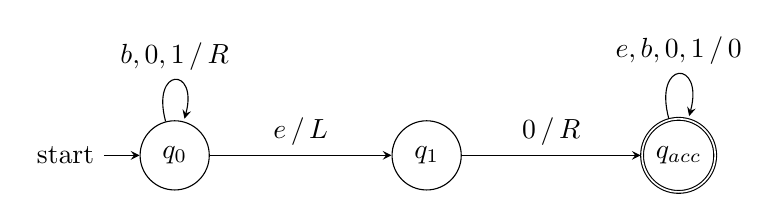
\begin{tikzpicture}[>=stealth, on grid, auto, node distance=3.2cm]
    \node[state, initial] (q0) {$q_0$};
    \node[state, right=of q0] (q1) {$q_1$};
    \node[state, accepting, right=of q1] (qacc) {$q_{acc}$};

    % scan to the right endmarker
    \path[->]
      (q0) edge[loop above] node {$b,0,1\,/\,R$} (q0)
      (q0) edge node {$e\,/\,L$} (q1);

    % check last symbol
    \path[->]
      (q1) edge node {$0\,/\,R$} (qacc)
      (qacc) edge[loop above] node {$e,b,0,1\,/\,0$} (qacc);
  \end{tikzpicture}

  \caption{A 2DFA with endmarkers recognizing
  $L=\{w\in\{0,1\}^*\mid w\text{ ends with }0\}$.
  Labels are “read symbol / head movement”, where $R$ means move right,
  $L$ means move left, and $0$ means stay.}
  \label{fig:2dfa-ends-with-0}
\end{figure}

The automaton first moves to the right until it reaches the right endmarker
$e$. It then moves one position to the left to inspect the last symbol of the
input word. If this symbol is $0$, the automaton moves right onto the
endmarker and enters the accepting state $q_{acc}$. If the last symbol is $1$,
no accepting transition is possible and the input is rejected.
Note that a 1DFA for the same language requires only two states,
as it can simply remember whether the last read symbol was $0$ or $1$.

\section{Why 2DFA Can Be Better Descriptions}

\subsection{Introduction}
In this section we present examples of regular languages where 2DFA can provide
more compact descriptions than one-way DFA and NFA, focusing
in particular on suffix-dependent and modular properties.
We will see that for certain languages the descriptive complexity reduces 
significantly when using two-way motion.

\subsection{Suffix-Dependent Languages}
We follow an example from Pighizzini \cite{pighizzini_2012_two_way} to prove 
the advantages of a 2DFA in contrast to a 1DFA for a specific suffix-dependent language.
We will also talk about 1NFA's in this context.
\begin{example}[Suffix language]
Let
\[
L_n := \{x \in \{0,1\}^* \; | \; \text{the n-th symbol from the right is 1}\}
\]
for $n \geq 1$.
\end{example}

When using two-way automata with both endmarkers, we can construct a 2DFA
with $n+3$ states, i.e. $O(n)$, for $L_n$ as follows:
\begin{itemize}
  \item The automaton starts in the initial state $q_0$ and moves right until
        it reads the right endmarker.
  \item Then it moves left $n$ positions, using states $q_1,\ldots,q_n$ to count
        the number of steps.
  \item Finally, it checks whether the current symbol is $1$ or $0$ and accepts
        or rejects accordingly using 2 states.
\end{itemize}
  
We conclude that a 2DFA with $O(n)$ states can recognize $L_n$.
Let's now consider a 1DFA for the same language.
One idea to construct such a 1DFA is the following: keep track of the last $n$ 
symbols with different states. 
Therefore we need states $\{0,1\}^n$, which gives us a total of $2^n$ states.
When reading a new symbol, the automaton updates its state to reflect the last $n$
accordingly. Accepting states are those where the first symbol of the last $n$ is $1$.

\begin{figure}[H]
  \centering
  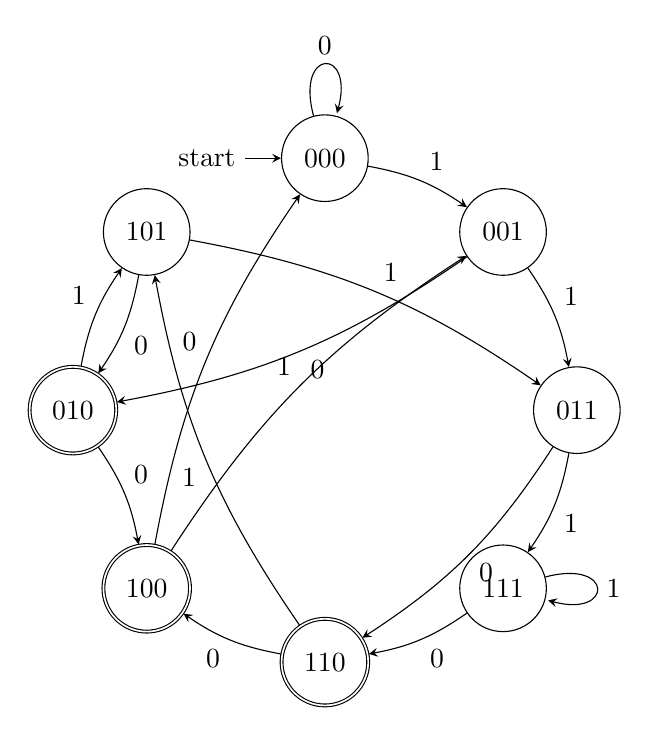
\begin{tikzpicture}[>=stealth, on grid, auto,
    every state/.style={minimum size=11mm}
  ]
    % circle radius
    \def\r{3.2cm}
  
    % nodes on a circle (clockwise)
    \node[state, initial] (000) at (90:\r) {$000$};
    \node[state]          (001) at (45:\r) {$001$};
    \node[state]          (011) at (0:\r) {$011$};
    \node[state]          (111) at (315:\r) {$111$};
    \node[state, accepting] (110) at (270:\r) {$110$};
    \node[state, accepting] (100) at (225:\r) {$100$};
    \node[state, accepting] (010) at (180:\r) {$010$};
    \node[state]          (101) at (135:\r) {$101$};
  
    % Transition rule: shift left and append input bit
    % 000
    \path[->] (000) edge[loop above] node {$0$} (000);
    \path[->] (000) edge[bend left=12] node {$1$} (001);
  
    % 001
    \path[->] (001) edge[bend left=12] node {$0$} (010);
    \path[->] (001) edge[bend left=12] node {$1$} (011);
  
    % 010
    \path[->] (010) edge[bend left=12] node {$0$} (100);
    \path[->] (010) edge[bend left=12] node {$1$} (101);
  
    % 011
    \path[->] (011) edge[bend left=12] node {$0$} (110);
    \path[->] (011) edge[bend left=12] node {$1$} (111);
  
    % 100
    \path[->] (100) edge[bend left=12] node {$0$} (000);
    \path[->] (100) edge[bend left=12] node {$1$} (001);
  
    % 101
    \path[->] (101) edge[bend left=12] node {$0$} (010);
    \path[->] (101) edge[bend left=12] node {$1$} (011);
  
    % 110
    \path[->] (110) edge[bend left=12] node {$0$} (100);
    \path[->] (110) edge[bend left=12] node {$1$} (101);
  
    % 111
    \path[->] (111) edge[bend left=12] node {$0$} (110);
    \path[->] (111) edge[loop right] node {$1$} (111);
  \end{tikzpicture}
  
  \caption{A 1DFA for $L_3$.
  The state stores the last three input symbols; accepting states are those whose leftmost bit is $1$.}
  \label{fig:dfa-L3-circle}
\end{figure}

We can conclude that we can construct a 1DFA for $L_n$ with $2^n$ states.
Next we will prove that this is asymptotically optimal.

\begin{theorem}
  Let
  \[
  L_n := \{x \in \{0,1\}^* \; | \; \text{the n-th symbol from the right is 1}\}
  \]
  for $n \geq 1$.
  Any 1DFA deciding $L_n$ requires $\Omega(2^n)$ states.
\end{theorem}

\begin{proof}
  Let M be the 1DFA deciding $L_n$ with transition function $\delta$ and starting state $q_0$.\\
  \\
  Let $u,v \in \{0,1\}^n$ be two different strings\\ and let $i \in \{0, \ldots, n-1\}$ 
  be the position in which the strings differ first (from the left).\\
  \\
  $w := 0^{n-1-i}$\\
  \\
  We can conclude that one of the words $uw, vw$ is accepted and the other is rejected.\\
  \\
  Assume $\delta(q_0, u) = \delta(q_0, v)$ then also $\delta(q_0, uw) = \delta(q_0, vw)$ because M is deterministic.\\
  $\Rightarrow$ contradiction $\Rightarrow$ $\delta(q_0, u) \neq \delta(q_0, v)$\\
  \\
  As a result, every string of length n requires a different state.\\
  $\Rightarrow$ $\Omega(2^n)$ different states.\\
\end{proof}

This proves that the 1DFA we constructed before is asymptotically optimal.
So we have shown that for the suffix-dependent language $L_n$ a 2DFA 
uses $O(n)$ states while a 1DFA, asymptotically optimal in terms of states, requires $2^n$ states.
The 2DFA has an exponential advantage in terms of descriptional complexity.

We can also construct a 1NFA for $L_n$ with $n+1$ states.
Nondeterminism allows us to guess the position that will become the n-th from the right.
This allows us to construct a 1NFA with only $n+1$ states, as shown in
Figure~\ref{fig:pighizzini-fig1-redraw}.

\begin{figure}[H]
  \centering
  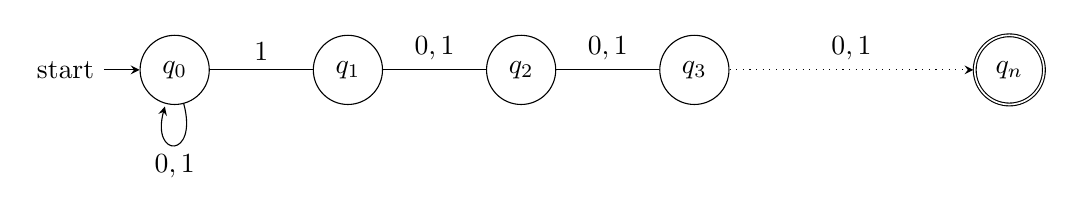
\begin{tikzpicture}[>=stealth, node distance=2.2cm, on grid, auto]
    \node[state, initial] (q0) {$q_0$};
    \node[state, right=of q0] (q1) {$q_1$};
    \node[state, right=of q1] (q2) {$q_2$};
    \node[state, right=of q2] (q3) {$q_3$};
    \node[state, accepting, right=4.0cm of q3] (qn) {$q_n$};
  
    % loop on q0
    \path (q0) edge[loop below] node {$0,1$} (q0);
  
    % transitions
    \path (q0) edge node {$1$} (q1);
    \path (q1) edge node {$0,1$} (q2);
    \path (q2) edge node {$0,1$} (q3);
  
    % dotted "..." segment to q_n
    \draw[->, dotted] (q3) -- node[above] {$0,1$} (qn);
  \end{tikzpicture}
  
  \caption{A 1NFA accepting the language
  $L_n$ (adapted from \cite[Fig.~1]{pighizzini_2012_two_way}).}
  \label{fig:pighizzini-fig1-redraw}
\end{figure}

So there is no improvement in terms of descriptional complexity when using a 2DFA
instead of a 1NFA for the suffix-dependent language $L_n$.

\subsection{Divisibility}
\begin{example}[Length divisible by $m$]
$L_m=\{\,w\in\{a\}^* \mid |w|\equiv 0 \ (\mathrm{mod}\ m)\,\}$.
\end{example}
Let's first prove that any one-way nondeterministic automaton for $L_m$ requires
at least $m$ states.

\begin{theorem}\label{thm:unary-mod-nfa-lb}
Any 1NFA deciding $L_m$ requires at least $m$ states.
Consequently, any 1DFA deciding $L_m$ requires at least $m$ states as well.
\end{theorem}

\begin{proof}
We use a fooling set to show a lower bound on 1NFA.
For $i=0,1,\ldots,m-1$ let $x_i:=a^i$ and $y_i:=a^{m-i}$, and define
\[
F:=\{(x_i,y_i)\mid i=0,\ldots,m-1\}.
\]
Then $x_i y_i=a^m\in L_m$ for all $i$.
If $i\neq j$, then
\[
x_i y_j = a^{\,i+m-j}
\]
has length $m+(i-j)$, which is not divisible by $m$ since $0<|i-j|<m$.
Hence $x_i y_j \notin L_m$ for all $i\neq j$, so $F$ is a fooling set of size $m$.
Therefore every 1NFA for $L_m$ has at least $m$ states.
Since 1DFA $\subset$ 1NFA the same lower bound holds for 1DFA.
\end{proof}

Note that in this example the lower bound for the states applies to both 1DFA and 1NFA.
There exists a standard 1DFA with $m$ states for $L_m$ (see, e.g., \cite{sipser,hopcroft}).
An example for $m=3$ is shown in Figure~\ref{fig:dfa-L3-mod}.

\begin{figure}[!htbp]
  \centering
  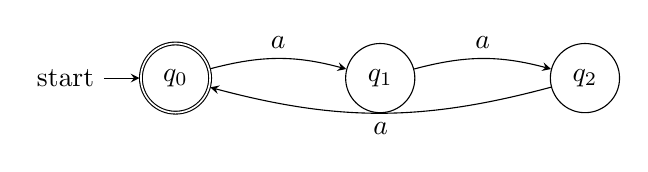
\begin{tikzpicture}[>=stealth, node distance=2.6cm, on grid, auto]
    \node[state, initial, accepting] (q0) {$q_0$};
    \node[state, right=of q0] (q1) {$q_1$};
    \node[state, right=of q1] (q2) {$q_2$};
  
    \path[->]
      (q0) edge[bend left=15] node {$a$} (q1)
      (q1) edge[bend left=15] node {$a$} (q2)
      (q2) edge[bend left=15] node {$a$} (q0);
  \end{tikzpicture}
  
  \caption{A 1DFA for $L_3$.}
  \label{fig:dfa-L3-mod}
\end{figure}

We can show that a 2DFA for $L_m$ can in some cases be significantly smaller.
Let $m = \prod_{i=1}^r p_i^{a_i}$ be a product of $r$ distinct primes 
$p_1 < p_2 < \cdots < p_r$ and exponents $a_i \in \mathbb{N}$ for $i \in \{1,\ldots,r\}$.
We can construct a 2DFA for $L_m$ with $\sum_{i=1}^r p_i^{a_i}$ states as follows:
In a first step the automaton counts the length of the input modulo $p_1^{a_1}$ by moving
from the first symbol from the left to the right endmarker. 
This requires $p_1^{a_1}$ states as in the standard modulo-m counter construction.
If the length is not divisible by $p_1^{a_1}$, the automaton rejects.
Then the automaton moves back to the left endmarker, while checking for divisibility
by $p_2^{a_2}$ in the same way.
After checking all $r$ prime power factors, the automaton accepts if and only if
all checks were successful
(cf.\ the general
succinctness discussion in \cite{pighizzini_2012_two_way}).

That example shows that with a 2DFA we can decrease the number of states from $\prod_{i=1}^r p_i^{a_i}$
to $\sum_{i=1}^r p_i^{a_i}$.
This is in contrast to the suffix dependent language from the previous example, 
where the 2DFA had no advantage over the 1NFA.

\section{Reductions: From 2DFA to One-Way Automata}

\subsection{Introduction}
At first sight, it may seem that allowing the head to move left increases the
power of finite automata beyond the regular languages. However, it is a classical
result that two-way deterministic finite automata recognize exactly the regular
languages; hence there is no increase in expressive power.

The equivalence of one-way and two-way finite automata was already known in the
late 1950s. A proof was presented at the Summer Institute of Symbolic Logic
in 1957 at Cornell University and was later referenced by Rabin and Scott in
their seminal paper \cite{rabin_scott_1959_finite_automata}.
A complete published proof was given by
Shepherdson in the same year \cite{shepherdson_1959_reduction}, based on
\emph{crossing sequences}. 
A different proof, using a subset construction, was later
presented by Vardi \cite{vardi_1989_note_reduction} in 1989.

In this section we present two constructions that simulate a given 2DFA by a
one-way automaton and analyze the resulting blow-up in the number of states.
We primarily follow Vardi's approach, which yields a one-way NFA for the
complement language. In addition, we briefly discuss Shepherdson's construction,
which yields an equivalent one-way DFA and is based on crossing sequences.

There are also proofs of the equivalence based on regular expressions; see, e.g.,
\cite{hulden_2015_two_way_to_one_way}. We do not cover this approach here.

\subsection{Reduction from 2DFA to 1NFA}
We follow the construction from Vardi's subset construction \cite{vardi_1989_note_reduction}.

\subsubsection{Lemma for Rejection Condition}
Before presenting the construction, we need a lemma.
\begin{lemma}[Vardi~\cite{vardi_1989_note_reduction}]
  \label{lem:rejection-condition}
  \emph{(Statement quoted verbatim from \cite{vardi_1989_note_reduction}.)}
  Let $A=(\Sigma,S,S_0,\rho,F)$ be a two-way automaton and let
  $w=a_0 a_1 \cdots a_n \in \Sigma^*$. The automaton $A$ rejects $w$ iff there
  exist sets $T_0,\ldots,T_{n+1} \subseteq S$ such that:
  \begin{enumerate}
    \item $S_0 \subseteq T_0$,
    \item $T_{n+1} \cap F = \emptyset$, and
    \item for every $0 \le i \le n$, every $s \in T_i$, and every transition
          $(s',k) \in \rho(s,a_i)$ with $i+k > 0$, we have $s' \in T_{i+k}$.
  \end{enumerate}
\end{lemma}
\begin{proof}
  ($\Rightarrow$) Suppose $A$ rejects $w$. For each $i \in \{0,\ldots,n+1\}$ define
  \[
  T_i := \{\, s \in S \mid \text{there exists a run of $A$ on $w$ that reaches a configuration }(s,i)\,\}.
  \]
  For every $s \in S_0$ there is a (trivial) run starting in configuration $(s,0)$,
  hence $S_0 \subseteq T_0$.
  Since $A$ rejects $w$, no accepting configuration at position $n+1$ is reachable.
  Therefore $T_{n+1} \cap F = \emptyset$.
  Finally, let $0 \le i \le n$, let $s \in T_i$, and let $(s',k) \in \rho(s,a_i)$
  with $i+k > 0$. By definition of $T_i$, there exists a run reaching $(s,i)$.
  Extending this run by one transition yields a run reaching $(s',i+k)$, hence
  $s' \in T_{i+k}$.
  
  ($\Leftarrow$) Suppose there exist sets $T_0,\ldots,T_{n+1} \subseteq S$ satisfying
  the three conditions. Assume for contradiction that $A$ accepts $w$.
  Then there exists a run $(s_0,j_0),\ldots,(s_m,j_m)$ with $s_0 \in S_0$, $j_0=0$,
  $j_m=n+1$, and $s_m \in F$.
  By (1), we have $s_0 \in T_{j_0}=T_0$. Using (3) inductively along the run, we get
  $s_i \in T_{j_i}$ for all $i$, and in particular $s_m \in T_{j_m} = T_{n+1}$.
  This contradicts (2) since $s_m \in F$. Hence, $A$ rejects $w$.
\end{proof}

\subsubsection{Construction of the 1NFA}
The properties of the lemma contain local conditions 
and can therefore be checked by a one-way automaton while scanning the input.
We implement these checks by constructing a 1NFA for the complement language.
Assume there is a 2DFA $A = (\Sigma,S,S_0,\rho,F)$, we then construct a 1NFA $B = (\Sigma,Q,Q_0,\delta,G)$ deciding $\Sigma^* \setminus L(A)$.
The state set $Q$ is
$2^S \cup (2^S)^2$, i.e., sets of states and pairs of sets of states. The
starting state set $Q_0$ is $\{\,T : S_0 \subseteq T \subseteq S\,\}$, i.e., the
collection of state sets that contain $S_0$. The accepting state set $G$ is
\[
\{\,T : T \cap F = \emptyset\,\} \;\cup\; \{\, (T,U) : U \cap F = \emptyset\,\},
\]
i.e., the collection of sets that do not intersect $F$ and pairs of sets whose
second component does not intersect $F$.

It remains to define the transition function $\delta$. We have $(T,U)\in\delta(T,a)$
if the following holds:
\begin{itemize}
  \item If $s \in T$ and $(t,0) \in \rho(s,a)$, then $t \in T$, and
  \item if $s \in T$ and $(t,1) \in \rho(s,a)$, then $t \in U$.
\end{itemize}

We have $(U,V)\in\delta((T,U),a)$ if the following holds:
\begin{itemize}
  \item If $s \in U$ and $(t,-1) \in \rho(s,a)$, then $t \in T$,
  \item if $s \in U$ and $(t,0) \in \rho(s,a)$, then $t \in U$, and
  \item if $s \in U$ and $(t,1) \in \rho(s,a)$, then $t \in V$.
\end{itemize}

\subsubsection{Correctness of the Construction}
The following lemma helps to proof the correctness of the construction.
\begin{lemma}\label{lem:correctness-of-construction}
  Let $A = (\Sigma,S,S_0,\rho,F)$ be a two-way automaton,
  $B = (\Sigma,Q,Q_0,\delta,G)$ be a 1NFA constructed as above and
  $w = a_0 a_1 \cdots a_n \in \Sigma^*$.
  Then $B$ accepts $w$ iff there exist sets $T_0,\ldots,T_{n+1} \subseteq S$
  satisfying the conditions lemma \ref{lem:rejection-condition}.
\end{lemma}

\begin{proof}
\noindent($\Rightarrow$)
Suppose $B$ accepts $w$. Then there exists an accepting path
$C_0,C_1,\ldots,C_{n+1}$ with $n \in \mathbb{N}$.

\medskip
\noindent
Set $T_0 := C_0 \in 2^S$.

\medskip
\noindent
Since $C_1 \in \delta(T_0,a_0)$, we have $C_1 = (T_0,T_1)$ with $T_1 \in 2^S$.

\medskip
\noindent
$\ldots$

\medskip
\noindent
Since $C_{n+1} \in \delta((T_{n-1},T_n),a_n)$, we have
$C_{n+1} = (T_n,T_{n+1})$ with $T_{n+1} \in 2^S$.

\medskip
\noindent
The accepting path rewritten:
\[
  T_0,\ (T_0,T_1),\ \ldots,\ (T_n,T_{n+1})
\]
with $T_i \in 2^S$.

\medskip
\noindent
We can now proof that $T_0,\ldots,T_{n+1}$ has the properties of lemma1:
\begin{enumerate}
  \item $T_0 \in Q_0 \Rightarrow S_0 \subset T_0$.
  \item $(T_n,T_{n+1}) \in G \Rightarrow T_{n+1} \cap F = \emptyset$.
  \item \textbf{($i=0$)} We have that $(T_0,T_1) \in \delta(T_0, a_0)$.
        For every $s \in T_0$ and $(s',k) \in \rho(s,a_i)$ with $i+k \geq 0$ the following holds:
        \[
          k \geq 0.
        \]
        If $k = 0$, then $s' \in T_0 = T_{i+k}$ (because of the construction of $B$).
        If $k = 1$, then $s' \in T_1 = T_{i+k}$ (because of the construction of $B$).
        Hence $s' \in T_{i+k}$.

        \medskip
        \noindent
        \textbf{($i>0$)} We have that $(T_i,T_{i+1}) \in \delta((T_{i-1},T_i),a_i)$.
        For every $s \in T_i$ and $(s',k) \in \rho(s,a_i)$ with $i+k \geq 0$ the following holds:
        \begin{itemize}
          \item if $k = -1$, then $s' \in T_{i-1} = T_{i+k}$ (because of the construction of $B$),
          \item if $k = 0$, then $s' \in T_{i+0} = T_{i+k}$ (because of the construction of $B$),
          \item if $k = 1$, then $s' \in T_{i+1} = T_{i+k}$ (because of the construction of $B$).
        \end{itemize}
        Hence $s' \in T_{i+k}$.
\end{enumerate}

\medskip
\noindent
$T_0,\ldots,T_{n+1}$ sequence exists as defined in Lemma \ref{lem:rejection-condition}.

\medskip
\noindent($\Leftarrow$)
Suppose there exists a sequence $T_0,\ldots,T_{n+1}$ as defined in Lemma \ref{lem:rejection-condition}.
We proof that $T_0,(T_0,T_1),\ldots,(T_n,T_{n+1})$ is a accepting path for $w$ in $B$.

\medskip
\noindent
We use property 1 $S_0 \subset T_0 \Rightarrow T_0 \in Q_0$.
We use property 2 $T_{n+1} \cap F = \emptyset \Rightarrow (T_n,T_{n+1}) \in G$.

\medskip
\noindent
Now we proof that there is a transition between the states:
\begin{itemize}
  \item \textbf{($i=0$)} $(T_0,T_1) \in \delta(T_0,a_0)$, because of property 3.
  \item \textbf{($i>0$)} $(T_i,T_{i+1}) \in \delta((T_{i-1},T_i),a_i)$, because of property 3.
\end{itemize}
\end{proof}

\begin{theorem}[Vardi~\cite{vardi_1989_note_reduction}]
  \emph{(Statement quoted verbatim from \cite{vardi_1989_note_reduction}.)}
  Let $A$ be a two-way automaton with $n$ states. Then there is a one-way automaton
  $B$ with $O(\exp n)$ states such that $L(B)=\Sigma^* - L(A)$. !!Its $O((\exp n)^2)$ states!!
\end{theorem}

\begin{proof}
  Let $A$ be a two-way automaton and let $B$ be the 1NFA obtained from $A$ by the
  construction above. Let $w \in \Sigma^*$.\newline
  $w \notin L(A)$ $\Leftrightarrow$ 
  There exists a sequence $T_0,\ldots,T_{n+1}$ satisfying the
  conditions of Lemma \ref{lem:rejection-condition} (Lemma \ref{lem:rejection-condition}). $\Leftrightarrow$
  $w \in L(B)$ (Lemma \ref{lem:correctness-of-construction}).
\end{proof}

\subsection{Reduction from 2DFA to 1DFA}
We follow the proof from Shepherdson \cite{shepherdson_1959_reduction} as presented by Vardi \cite{vardi_1989_note_reduction}.
The full proof is quite long and technical, so we only outline the main idea here.
Let $A=(\Sigma,S,S_0,\rho,F)$ be a two-way automaton and let
$w=a_0 a_1 \cdots a_n \in \Sigma^*$.
We define a A-label as a pair $(s_1,s_2)$ where $s_1,s_2 \in S$, which represents a
run from $s_1$ to $s_2$.
An A-labeling is a sequence of sets of A-labels, one set for each position in the input:
\[
m_0, m_1, \ldots, m_n \quad \text{with } m_i \subseteq S \times S.
\]
Intuitively, when there is an A-label $(s_1,s_2)$ in $m_i$, then there is a run of $A$ that
starts in state $s_1$ at position $i$ on word $w$ and ends in state $s_2$ at position $i$.
This run is guarenteed to never visit position $i+1$.

As you may have noticed, with a given A-labeling we dont have to go 
to the left. Assume we are at position i in state $s$ and we have to go to the left.
We can look at the A-labels in $m_{i}$ to find a label $(s, s')$.
Instead of going to the left, we can jump to state $s'$ at position $i$.
This way we can simulate the two-way motion of $A$ with one-way motion.

Note that at at position $i$ and for a given state $s_1$ there can be multiple
A-labels $(s_1,s_2)$ in $m_i$ with different $s_2$.

The difficult part is to create a one-way automaton that constructs valid A-labelings
while reading the input from left to right. The automaton has to generate the 
A-labeling on the fly. Such that at position $i$ it has generated $m_0, m_1, \ldots, m_i$.
The automaton has to make sure that the A-labels are consistent with each other
and with the transition function $\rho$ of $A$.
The details are quite technical and we refer to the original paper by Shepherdson
\cite{shepherdson_1959_reduction} or the presentation by Vardi \cite{vardi_1989_note_reduction}
for more information.

The following theorem summarizes the result of the construction.

\begin{theorem}
  \emph{(Statement quoted verbatim from Vardi \cite{vardi_1989_note_reduction}.)}
  Let $A$ be a two-way automaton with $n$ states. Then there is a one-way
  deterministic automaton $B$ with $O(\exp n)$ states such that $L(B)=L(A)$.
  \label{thm:2dfa-to-1dfa}  
\end{theorem}

\subsection{State Blow-Up and Complexity Discussion}
The construction in Chapter 5.2 by Vardi \cite{vardi_1989_note_reduction} yields a 1NFA with
$O((\exp n)^2)$ states for a given 2DFA with $n$ states.
The 1NFA automata decides the complement language.
We can convert the 1NFA to a 1DFA, which results into a exponentially blow-up of states.
The resulting 1DFA has $O(\exp((\exp n)^2))$ states and decides the complement language.
We can flip the accepting and non-accepting states to get a 1DFA for the original language, 
without increasing the number of states. This trick doesnt work for the 1NFA, because of nondeterminism.
As a result we get a 1DFA with $O(\exp((\exp n)^2))$ states for a given 2DFA with $n$ states.

The construction in Chapter 5.3 by Vardi \cite{vardi_1989_note_reduction} based on Shepherdson \cite{shepherdson_1959_reduction} with crossing sequences yields a 1DFA with
$O(\exp n)$ states for a given 2DFA with $n$ states.

To solve the task: "Given a two-way automata with n states, construct an equivalent one-way automata."
Theorem \ref{thm:2dfa-to-1dfa} is the better choice, because of less state blow-up.

Also the task: "Given a two-way automata with n states, construct a one-way automata deciding the complement."
Theorem \ref{thm:2dfa-to-1dfa} is the better choice, because $O(\exp n)$ is better then a blowup of $O(\exp(n)^2)$.

\subsection{Worked Example}
We will now present a small example of a 2DFA and outline how the construction from
Vardi \cite{vardi_1989_note_reduction} would work on this example.
The concrete construction is explained in Chapter 5.2.
Let $A=(\Sigma,S,S_0,\rho,F)$ be a 2DFA with

\section{Conclusion}

In this report we introduced two-way finite automata and
compared them with classical one-way models. We first established the formal
definitions and basic properties of two-way automata and then investigated their
descriptive advantages over one-way finite automata. Although allowing the read head to move in both
directions might at first suggest a higher expressive power, we have seen that
2DFA recognize exactly the class of regular languages and therefore do not extend
the expressive power of finite automata.

The first main topic was about \emph{descriptional complexity}. We presented
examples of regular languages for which two-way motion leads to significantly more
compact automata. In particular, suffix-dependent languages and modular
(divisibility) languages illustrate that a 2DFA may require fewer
states than a corresponding 1DFA. In the case of suffix-dependent languages, we
constructed a 2DFA with a linear number of states, while any equivalent 1DFA
requires exponentially many states. Also we showed an equivalent 1NFA with a linear
number of states, demonstrating that nondeterminism is as powerful as
two-way motion for this language family. For modular languages, we presented a
2DFA construction with $\sum_i p_i^{a_i}$ states for a modulus
$m=\prod_i p_i^{a_i}$, while any equivalent one-way automaton requires at least
$\prod_i p_i^{a_i}$ states. This descriptive complexity gap also holds
for one-way nondeterministic automata.

Another main topic of this report was the \emph{expressive complexity} of two-way finite automata.
To show that the additional head movement does not increase expressive power, we
discussed classical reductions from 2DFA to one-way automata. We followed Vardi's
subset-style construction \cite{vardi_1989_note_reduction}, 
which yields a one-way NFA for the complement language,
and outlined Shepherdson's crossing-sequence construction 
(\cite{vardi_1989_note_reduction},\cite{shepherdson_1959_reduction}), 
which produces an
equivalent one-way DFA. These two approaches highlight different trade-offs: while
Vardi's proof is easier to understand, Shepherdson's method achieves a more
favorable asymptotic bound on the number of states in the resulting deterministic
automaton.

Several aspects were beyond the scope of this report. These include alternative
equivalence proofs based on regular expressions \cite{hulden_2015_two_way_to_one_way}, 
restricted variants of two-way
automata such as models with nondeterminism only at the endmarker position \cite{pighizzini_2012_two_way}, 
and further language families that exhibit gaps in descriptional complexity.
\bibliographystyle{plain}
\bibliography{references}

\appendix

\end{document}
